
%% report_template.tex
%% V1.0
%% 2012-03-16
%% by Jesper Pedersen Notander
%% See:
%% http://www.cs.lth.se/jesper_pedersen_notander
%% for current contact information.
%%
%% This is a template file contaning instructions and a skeleton outline
%% for the final report in the course ETSA05: Software Engineering
%% Process - Soft Issues, given by the Department of Computer Science at
%% Lund University, Sweden.
%%
%% This template requires IEEEtran.cls, written by Michael Shell, version
%% 1.7 or later.
%%
%% Support sites:
%% http://www.cs.lth.se/etsa05/
%% http://www.ieee.org/

%%*************************************************************************
%% Legal Notice:
%% This code is offered as-is without any warranty either expressed or
%% implied; without even the implied warranty of MERCHANTABILITY or
%% FITNESS FOR A PARTICULAR PURPOSE!
%%
%% User assumes all risk.
%%
%% In no event shall Lund University or any contributor to this code be
%% liable for any damages or losses, including, but not limited to,
%% incidental, consequential, or any other damages, resulting from the use
%% or misuse of any information contained here.
%%
%% All comments are the opinions of their respective authors and are not
%% necessarily endorsed by Lund University.
%%
%% This work is distributed under the LaTeX Project Public License (LPPL)
%% ( http://www.latex-project.org/ ) version 1.3, and may be freely used,
%% distributed and modified. A copy of the LPPL, version 1.3, is included
%% in the base LaTeX documentation of all distributions of LaTeX released
%% 2003/12/01 or later.
%%
%% Retain all contribution notices and credits.
%% ** Modified files should be clearly indicated as such, including  **
%% ** renaming them and changing author support contact information. **
%%
%% File list of work: report_template.tex
%%*************************************************************************


\documentclass[conference]{IEEEtran}
\usepackage{graphicx}
% If IEEEtran.cls has not been installed into the LaTeX system files,
% manually specify the path to it like:
% \documentclass[conference]{../sty/IEEEtran}

\begin{document}

\title{Title}

% Leave as is to ensure anonymous grading.
\author{
\IEEEauthorblockN{ANONYMOUS AUTHOR}
\IEEEauthorblockA{Examination in DIT348 Software Development Methodologies\\
Department of Computer Science and Engineering\\
University of Gothenburg\\
Gothenburg, Sweden}}

\maketitle

\begin{abstract}
This document is a template. The various components of your essay (title, headings, etc.) are already defined here. Please note that the headings must NOT change unless explicitly stated below. That is, you MUST use the predefined headings. Make sure to retain font sizes, line spacing, column width, and margins. Not following this template in either structure or layout will lead to a FAIL. Remember: the criteria for attaining the grades are defined in the course syllabus. To get a pass with distinction (5), you need to solve the bonus task (Section~\ref{sec:bonus_task}). Please replace this abstract with your own text, briefly state what this report is about, and summarize the key take-aways.
\end{abstract}

\section{Introduction}
This template is a document that provides the predefined outline of your essay. You must use the predefined outline and you must NOT change any headings in the outline unless otherwise noted in the instructions. It is important to note that you have a page limit of \textbf{six pages} for your report, hence it is important to decide how much should be analyzed, discussed, and written for each section.

The introduction section should be used to introduce Software Processes and Software Process Improvement (SPI) in general and to introduce the purpose and context of this report.
To set the stage, describe in 1--2 sentences what a software process is.
Afterwards, explain in 1--2 sentences what software process improvement (SPI) is.

The Abstract, Introduction and Summary sections play a smaller part in the assessment. Therefore, most of your effort (and space in the essay) should be put into Sections \ref{sec:process}, \ref{sec:experiences}, \ref{sec:spi-techniques}, \ref{sec:proposal}, \ref{sec:implementation}, and \ref{sec:redesign}.

Please note that it is important that you use peer-reviewed and relevant references when you describe, reflect, and discuss aspects of SPI throughout the entire take-home exam. Whenever referencing a paper, make sure that it is clear why you referenced it and how it contributes to your argument.

Since some of the work performed in the course is group work, some overlap between members of the same group is expected. You are encouraged to reuse the joint work you did in class in some sections if a corresponding statement is made in that section. However, this is an individual written exam rather than a group exam. Therefore, make sure that different members of the same group do not use the same text. Verbatim copying is not permissible.

This section must be worked on individually.

\section{Process Defined for the Scrum Workshop}
\label{sec:process}
Describe the process you defined for the Scrum Lego Workshop. Explain whether you chose to apply Scrum, User Story Practice, and Incremental Delivery. Give reasons for why you did or did not use elements from these three practices.

You can use the results of the first assignment and in-class sessions. While it is okay if members of the same group provide similar answers based on your common process definition, each group member has to formulate this section independently.

\section{Experiences in the Scrum Workshop}
\label{sec:experiences}
In this section, you should describe your experiences during the first Scrum Lego workshop. Put a special focus on how you and your group were using the process, which parts of the process worked well, and which parts of the process did not work well. For the latter part, analyze the reasons that caused problems. Use at least three references to the literature (e.g., \cite{CaterSteel2006}, \cite{Abrahamsson2002}) to identify if the issues you encountered are general problems or specific to your effort.

You can use the results of the second assignment. While it is okay if members of the same group provide similar answers, each group member has to formulate this section independently.

If you did not attend the Scrum Lego workshop, find literature that describes development efforts and the problems within them. Describe and analyze at least five such papers, which problems have been encountered, what the underlying reasons for the problems were, and whether the issues encountered were general or not. If you go with this option, use the heading ``Reported Experiences in Development Efforts'' for this section.


\begin{figure*}
	\centering
	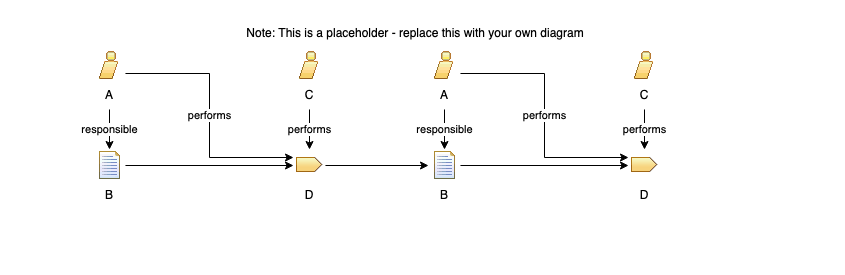
\includegraphics[width=0.9\textwidth]{placeholder_diagram}
	\caption{Placeholder diagram showing your envisioned process}
	\label{fig:placeholderdiagram}
\end{figure*}
\section{Software Process Improvement Techniques}
\label{sec:spi-techniques}
Provide at least three examples of SPI methods/models/techniques (for an overview, see, e.g., \cite{Pettersson2008}). Describe each of them together with at least one advantage and one disadvantage.
Relate each of those methods/models/techniques to the problems you encountered and described in Section~\ref{sec:experiences}.
Explain whether they are applicable to your issues and why.

This section must be worked on individually.

\section{SPI Proposal for future Scrum Development Efforts}
\label{sec:proposal}
In this section, you should discuss and explain the concrete SPI steps that you suggest to take in order to improve the process you applied during the first Scrum Lego Workshop. First, define at least three goals for an SPI proposal based on what you wrote in Section~\ref{sec:experiences}. Second, define questions and metrics you connect to those goals.
Then, use the tools that were introduced in the course (e.g., GQM or CMMI roadmaps) to define at least two concrete improvement steps per goal. Also, include a plan for how to measure whether your improvement effort was successful. Be careful to reference the corresponding literature when you mention a tool for the first time.

You can use the results of any of the assignments and in-class exercises for this section. While it is okay if members of the same group provide similar answers, each group member has to formulate this section independently.

If you did not attend the Scrum Lego workshop, base your proposal on your analysis in Section~\ref{sec:experiences}. Follow the same guidelines as above for the Scrum Lego workshop. If you go with this option, use the heading ``SPI Proposal for an Industrial Case Study'' for this section.

\section{Implementation of an SPI Initiative}
\label{sec:implementation}
You implemented an SPI initiative in the second workshop.
Give a summary of at least two actual changes that were implemented by your group. These might differ from your original proposal, since not all of your ideas from the proposal might be feasible. Describe at least two effects of those changes and analyze why these effects manifested themselves.
For the selected changes, provide at least one example of concrete measurements that you have made.

This section should contain the overall result for the entire group. Still, each group member has to formulate this section independently.

If you did not attend the Lego workshops, this section may be dedicated to a discussion of challenges in SPI projects. Find at least four relevant references that mention and analyze challenges and compile an overview of what has been observed in the literature. Relate these challenges to empirical studies that have been published and to your personal experience. Identify the SPI techniques that might help to overcome these challenges. Critically discuss the solution approaches from the papers.

\section{Redesign of the Software Process}
\label{sec:redesign}
After reflecting on the SPI experiences, think about how you would design your process for the Lego workshop if you could do it again.
Create a SPEM 2.0 diagram and replace Figure~\ref{fig:placeholderdiagram} with it.
Briefly describe at least the key task definitions, role definitions, and work product definitions that you aim to use, with 1--2 sentences per definition.

This section must be worked on individually.

\section{Bonus Task: Scrum of Scrums}
\label{sec:bonus_task}
This task needs to be solved to get a 5 (pass with distinction).
Note that to get a 5, all other tasks need to be at a level that fulfill the criteria for a 4.
The bonus task cannot be used to pass the exam if you would fail it based on the other tasks.
It cannot be used to improve a 3 (pass) either.

In the workshops, you observed many issues that related to inter-team coordination. One way to address those issues is to have more frequent Scrum of Scrum meetings. Another way to solve them is to have coordination artifacts that create a common understanding between different teams. Find at least three different peer-reviewed sources in the literature that discuss inter-team coordination and/or Scrum of Scrum meetings. Explain at least two challenges that have been reported connected to Scrum of Scrum meetings. Explain and justify whether you would recommend big companies to rely on frequent Scrum of Scrum meetings or whether you think other mechanisms are better for inter-team coordination. 


If you decide to submit the bonus task, you get 1/2 page for it. The new page limit will be 6.5 pages.
\section{Summary and Lessons Learned}
\label{sec:summary}
In the summary section, you should briefly summarize what your report is about and present your main findings/consequences.

This section must be worked on individually.

% This is used to generate the references section. See mybibfile.bib for the bib sources.
\bibliographystyle{IEEEtran}
\bibliography{mybibfile}


% If the bib file doesn't work for you, you can also define the references section like this:
%\begin{thebibliography}{1}
%	
%	\bibitem{CaterSteel2006}
%	A.~Cater-Steel, M.~Toleman, and T.~Rout, ``Process Improvement for Small Firms: An Evaluation of the RAPID Assessment-Based Method''. Information and Software Technology, vol.~48, no.~5, pp.~323- 334, 2006.
%	
%	\bibitem{Abrahamsson2002}
%	P.~Abrahamsson and K.~Kautz, ``Personal Software Process: Classroom Experiences from Finland''. Proc.~Software Quality -- ESCQ '02, pp.~175-85, Springer, 2002.
%	
%	\bibitem{Pettersson2008}
%	F.~Pettersson, M.~Ivarsson, T.~Gorschek, and P.~{\"O}hman, ``A practitioner's guide to light weight software process assessment and improvement planning''. Journal of Systems and Software, 81(6), pp. 972-995, 2008
%	
%\end{thebibliography}
\end{document}


